\chapter{Modelo de ejecución de funciones y recursión}

\section{La pila de ejecución de las funciones}

% TODO:
% Esta sección debería estar en un capítulo muy anterior.  Estos conceptos
% los venimos usando desde bastante antes de ver objetos.

Si miramos el siguiente segmento de código y su ejecución podemos comprobar
que, pese a tener el mismo nombre, la variable de \lstinline!x! de la función
\lstinline!f! y la variable de \lstinline!x! de la función \lstinline!g! no
tienen nada que ver: una y otra se refieren a valores distintos, y modificar
una no modifica a la otra.

\begin{codigo-python-sn}
def f():
    x = 50
    a = 20
    print("En f, x vale", x)

def g():
    x = 10
    b = 45
    print("En g, antes de llamar a f, x vale", x)
    f()
    print("En g, después de llamar a f, x vale", x)
\end{codigo-python-sn}

Esta es la ejecución de \lstinline!g()!:

\begin{codigo-python-sn}
>>> g()
En g, antes de llamar a f, x vale 10
En f, x vale 50
En g, después de llamar a f, x vale 10
\end{codigo-python-sn}

Este comportamiento lo dimos por sentado desde el principio, pero nunca nos
detuvimos a pensar por qué sucede.  Vamos a ver en esta sección cómo se
ejecutan las llamadas a funciones, para comprender cuál es la razón de este
comportamiento.

Cada función tiene asociado por un lado un código (el texto del programa)
que se ejecutará, y por el otro un conjunto de variables que le son propias
(en este caso \lstinline!x! y \lstinline!a! se asocian con \lstinline!f! y
\lstinline!x! y \lstinline!b! se asocian con \lstinline!g!) y que no se
confunden entre sí pese a tener el mismo nombre. No debería llamarnos la
atención, ya que después de todo conocemos a muchas personas que tienen el
mismo nombre.

Estos nombres asociados a una función los va {\it descubriendo} el intérprete de
Python a medida que va ejecutando el programa (hay otros lenguajes en los
que los nombres se descubren todos juntos antes de iniciar la ejecución).

La ejecución del programa se puede modelar por el siguiente diagrama, en el
cual los nombres asociados a cada función se encerrarán en una caja o {\it
marco}:

\newcommand{\currentframe}{\raisebox{1pt}{\tiny$\blacktriangleright$\normalsize} }

\begin{enumerate}

\item  \verb|g()   | \hspace{1.5cm}
	\begin{tabular}{r|r|}
	\hline
	\currentframe \verb|g|&\phantom{\verb|x| $\rightarrow$ 10} \\
	\hline
	\end{tabular}

\item  \verb|x = 10| \hspace{1.5cm}
	\begin{tabular}{r|r|}
	\hline
	\currentframe \verb|g|& \verb|x| $\rightarrow$ 10 \\
	\hline
	\end{tabular}

\item  \verb|b = 45| \hspace{1.5cm}
	\begin{tabular}{r|r|}
	\hline
	\currentframe \verb|g|& \verb|x| $\rightarrow$ 10 \\
	        & \verb|b| $\rightarrow$ 45 \\
	\hline
	\end{tabular}

\item  \verb|print | \hspace{1.5cm}
	\begin{tabular}{r|r|}
	\hline
	\currentframe \verb|g|& \verb|x| $\rightarrow$ 10 \\
	             & \verb|b| $\rightarrow$ 45 \\
	\hline
	\end{tabular}
	\hspace{1cm}
	\begin{tabular}{l}
	Imprime: \\
	{\small\tt En g, antes de llamar a f, x vale 10}
	\end{tabular}

\item  \verb|f()   | \hspace{1.5cm}
	\begin{tabular}{r|r|}
	\hline
	\currentframe \verb|f|&\\
	\hline
	\hline
	\verb|g|& \verb|x| $\rightarrow$ 10 \\
	        & \verb|b| $\rightarrow$ 45 \\
	\hline
	\end{tabular}

\item  \verb|x = 50| \hspace{1.5cm}
	\begin{tabular}{r|r|}
	\hline
	\currentframe \verb|f|& \verb|x| $\rightarrow$ 50 \\
	\hline
	\hline
	\verb|g|& \verb|x| $\rightarrow$ 10 \\
	        & \verb|b| $\rightarrow$ 45 \\
	\hline
	\end{tabular}

\item  \verb|a = 20| \hspace{1.5cm}
	\begin{tabular}{r|r|}
	\hline
	\currentframe \verb|f|& \verb|x| $\rightarrow$ 50 \\
	             & \verb|a| $\rightarrow$ 20 \\
	\hline
	\hline
	\verb|g|& \verb|x| $\rightarrow$ 10 \\
	        & \verb|b| $\rightarrow$ 45 \\
	\hline
	\end{tabular}

\item  \verb|print | \hspace{1.5cm}
	\begin{tabular}{r|r|}
	\hline
	\currentframe \verb|f|& \verb|x| $\rightarrow$ 50 \\
	             & \verb|a| $\rightarrow$ 20 \\
	\hline
	\hline
	\verb|g|& \verb|x| $\rightarrow$ 10 \\
	        & \verb|b| $\rightarrow$ 45 \\
	\hline
	\end{tabular}
	\hspace{1cm}
	\begin{tabular}{l}
	Imprime: \\
	{\small\tt En f, x vale 50}
	\end{tabular}

\item  \verb|print | \hspace{1.5cm}
	\begin{tabular}{r|r|}
	\hline
    \currentframe \verb|g|& \verb|x| $\rightarrow$ 10 \\
	        & \verb|b| $\rightarrow$ 45 \\
	\hline
	\end{tabular}
	\hspace{1cm}
	\begin{tabular}{l}
	Imprime: \\
	{\small\tt En g, despues de llamar a f, x vale 10}
	\end{tabular}

\item  \verb|      | \hspace{1.5cm}
	\begin{tabular}{r|r|}
	\hline
	\currentframe pila vacía\\
	\hline
	\end{tabular}

\end{enumerate}

Se puede observar que:
\begin{itemize}

\item Cuando se invoca a \lstinline|g|, se arma un {\it marco} vacío para
contener las referencias a las variables asociadas con \lstinline|g|. Ese
marco se apila sobre una {\it pila vacía}. El marco que está en el tope de la
pila es el {\it marco actual} y se marca con \currentframe en el diagrama.

\item Cuando se ejecuta dentro de \lstinline|g| la invocación
\lstinline|f()| (en el paso 5) se {\it apila} un marco vacío que va a alojar
las variables asociadas con \lstinline|f|, que pasa a ser el marco actual,
y se transfiere el control del
programa a la primera instrucción de \lstinline|f|.  El marco de
\lstinline|g| queda debajo del tope de la pila, y por lo tanto el
intérprete no lo ve.

\item Mientras se ejecuta \lstinline|f|, el intérprete busca los
valores que necesita usando el marco que está en el tope de la pila. Si alguna
línea de código de |f| intentara acceder a una variable llamada |b|, el
intérprete no la encontraría y lanzaría una excepción.

\item Después de ejecutar 8, se encuentra el final de la ejecución de
\lstinline|f|.  Se desapila el marco de \lstinline|f| y reaparece el marco
de \lstinline|g| en el tope de la pila. Sigue ejecutando \lstinline|g| a
partir de donde se suspendió por la invocación a \lstinline|f|.
\lstinline|g| sólo ve su marco en el tope de la pila.

\item Después de ejecutar 9, se encuentra el final de la ejecución de
\lstinline|g|.  Se desapila el marco de \lstinline|g| y queda la pila vacía.

\end{itemize}

El {\bf ámbito de definición} de una variable está constituido por todas las
partes del programa desde donde esa variable {\it es visible}.

\section{Pasaje de parámetros}

Un parámetro es una variable más dentro del marco de una función.
Sólo hay que tener en cuenta que si en la invocación se le pasa
un valor a ese parámetro, en el marco inicial esa variable ya aparecerá
ligada a un valor. Analicemos el siguiente código de ejemplo:

\begin{codigo-python-sn}
def fun1(a):
    print(a + 1)

def fun2(b):
    fun1(b + 5)
    print("Volvio a fun2")
\end{codigo-python-sn}

Con la siguiente ejecución:

\begin{codigo-python-sn}
>>> fun2(43)
49
Volvio a fun2
\end{codigo-python-sn}

En este caso, la ejecución se puede representar de la siguiente manera:

% Tablas de ejecución
\begin{enumerate}

\item  \verb|fun2(43)  | \hspace{1.5cm}
	\begin{tabular}{r|r|}
	\hline
	\currentframe \verb|fun2|&\verb|b| $\rightarrow$ 43\\
	\hline
	\end{tabular}

\item  \verb|fun1(b+5) | \hspace{1.5cm}
	\begin{tabular}{r|r|}
	\hline
	\currentframe \verb|fun1|&\verb|a| $\rightarrow$ 48\\
	\hline
	\hline
	\verb|fun2|&\verb|b| $\rightarrow$ 43\\
	\hline
	\end{tabular}

\item  \verb|print(a+1)| \hspace{1.5cm}
	\begin{tabular}{r|r|}
	\hline
	\currentframe \verb|fun1|&\verb|a| $\rightarrow$ 48\\
	\hline
	\hline
	\verb|fun2|&\verb|b| $\rightarrow$ 43\\
	\hline
	\end{tabular}
	\hspace{1cm}
	\begin{tabular}{l}
	Imprime: \\
	{\small\tt 49}
	\end{tabular}

\item  \verb|print     | \hspace{1.5cm}
	\begin{tabular}{r|r|}
	\hline
	\currentframe \verb|fun2|&\verb|b| $\rightarrow$ 43\\
	\hline
	\end{tabular}
	\hspace{1cm}
	\begin{tabular}{l}
	Imprime: \\
	{\small\tt Volvio a fun2}
	\end{tabular}

\item  \verb|          | \hspace{1.5cm}
	\begin{tabular}{r|r|}
	\hline
	\currentframe pila vacía\\
	\hline
	\end{tabular}

\end{enumerate}

Cuando se pasan objetos como parámetros, las dos variables hacen referencia al {\it mismo}
objeto. Eso significa que si el objeto pasado es mutable, cualquier modificación que
la función invocada realice sobre su parámetro se reflejará en el argumento de la función llamadora,
como se puede ver en el siguiente ejemplo:

\begin{codigo-python-sn}
def modif(lista):
    lista[0] = 5

def main():
    ls = [1, 2, 3, 4]
    print(ls)
    modif(ls)
    print(ls)
\end{codigo-python-sn}

Y esta es la ejecución:
\begin{codigo-python-sn}
>>> main()
[1, 2, 3, 4]
[5, 2, 3, 4]
\end{codigo-python-sn}

\begin{itemize}

\item Cuando se invoca a \lstinline|modif(ls)| desde \lstinline|main|, el
esquema de la pila es
el siguiente:

\verb|modif(ls)   | \hspace{1.5cm}
	\begin{tabular}{r|l||l|}
	\hline
	\currentframe \verb|modif|&\verb|lista|\tikzmark{ls1}\verb|  | & \\
	\cline{1-2}
	\cline{1-2}
	              \verb|main|&\verb|ls|\tikzmark{ls2}\verb|     | & \multirow{-2}{*}{\verb|  |\tikzmark{t}\verb|[1, 2, 3, 4]|}\\
	\hline
	\end{tabular}
\tikz[overlay,remember picture] \draw[-latex,thick] ($(ls1.north east)$) -- ($(t.north)$);
\tikz[overlay,remember picture] \draw[-latex,thick] ($(ls2.north east)+(0,-0.04)$) -- ($(t)$);

\item Cuando se modifica la lista desde \lstinline|modif|, el esquema de la
pila es el siguiente:

\verb|lista[0] = 5| \hspace{1.5cm}
	\begin{tabular}{r|l||l|}
	\hline
	\currentframe \verb|modif|&\verb|lista|\tikzmark{ls1}\verb|  | & \\
	\cline{1-2}
	\cline{1-2}
	              \verb|main|&\verb|ls|\tikzmark{ls2}\verb|     | & \multirow{-2}{*}{\verb|  |\tikzmark{t}\verb|[5, 2, 3, 4]|}\\
	\hline
	\end{tabular}
\tikz[overlay,remember picture] \draw[-latex,thick] ($(ls1.north east)$) -- ($(t.north)$);
\tikz[overlay,remember picture] \draw[-latex,thick] ($(ls2.north east)+(0,-0.04)$) -- ($(t)$);

\item Cuando la ejecución vuelve a \lstinline|main|, \lstinline!ls!
seguirá apuntando a la lista \lstinline|[5, 2, 3, 4]|.

\end{itemize}

En cambio, cuando el parámetro cambia la referencia que se le pasó por una
referencia a otro objeto, la función |main| no se entera:

\begin{codigo-python-sn}
def cambia_ref(lista):
    lista = [5, 2, 3, 4]

def main():
    ls = [1, 2, 3, 4]
    print(ls)
    cambia_ref(ls)
    print(ls)
\end{codigo-python-sn}

\begin{codigo-python-sn}
>>> main()
[1, 2, 3, 4]
[1, 2, 3, 4]
\end{codigo-python-sn}

\begin{itemize}

\item Cuando se invoca a \lstinline|cambia_ref(ls)| desde
\lstinline|main|, el esquema de la pila es el siguiente:

\verb|cambia_ref() | \hspace{1.5cm}
	\begin{tabular}{r|l||l|}
	\hline
	\currentframe \verb|cambia_ref|&\verb|lista|\tikzmark{ls1}\verb|  | & \\
	\cline{1-2}
	\cline{1-2}
	              \verb|main|&\verb|ls|\tikzmark{ls2}\verb|     | &
                    \multirow{-2}{*}{\verb|  |\tikzmark{t}\verb|[1, 2, 3, 4]|}\\
	\hline
	\end{tabular}
\tikz[overlay,remember picture] \draw[-latex,thick] ($(ls1.north east)$) -- ($(t.north)$);
\tikz[overlay,remember picture] \draw[-latex,thick] ($(ls2.north east)+(0,-0.04)$) -- ($(t)$);

\item Cuando se cambia referencia a la lista desde \verb|cambia_ref|, {\bf se crea
una nueva instancia de lista}, y el esquema de la pila es el siguiente:

\verb|lista = [...]| \hspace{1.5cm}
	\begin{tabular}{r|l||l|}
	\hline
	\currentframe \verb|cambia_ref|&\verb|lista|\tikzmark{ls1}\verb|  | &
        \verb|  |\tikzmark{t1}\verb|[5, 2, 3, 4]|\\
	\cline{1-2}
	\cline{1-2}
	              \verb|main|&\verb|ls|\tikzmark{ls2}\verb|     | &
        \verb|  |\tikzmark{t2}\verb|[1, 2, 3, 4]|\\
	\hline
	\end{tabular}
\tikz[overlay,remember picture] \draw[-latex,thick] ($(ls1.north east)+(0,-0.04)$) -- ($(t1.north west)+(0,-0.04)$);
\tikz[overlay,remember picture] \draw[-latex,thick] ($(ls2.north east)+(0,-0.04)$) -- ($(t2.north west)+(0,-0.04)$);

\item Cuando la ejecución vuelve a \lstinline|main|, \lstinline!ls!
seguirá apuntando a la lista \lstinline|[1, 2, 3, 4]|.

\end{itemize}

\section{Devolución de resultados}

Finalmente, para completar los distintos seguimientos, debemos tener en
cuenta que los resultados que devuelve la función invocada, se {\it reciben}
en la expresión correspondiente de la función invocante.

\begin{codigo-python-sn}
def cuad(valor):
    c = valor * valor
    return c

def main():
    c = cuad(6)
    print(c)
\end{codigo-python-sn}

En este caso, si hacemos el seguimiento de la funcion invocada:
\begin{codigo-python-sn}
>>> main()
36
\end{codigo-python-sn}

Veremos algo como lo siguiente:

% Tablas de ejecución
\begin{enumerate}

\item \makebox[5cm][l]{\verb|main()|}
	\begin{tabular}{r|l|}
	\hline
	\currentframe \verb|main| & \phantom{\verb|valor| $\rightarrow$ 5} \\
	\hline
	\end{tabular}

\item \makebox[5cm][l]{\verb|c = cuad(6)|}
	\begin{tabular}{r|l|}
	\hline
	\currentframe \verb|main| & \phantom{\verb|valor| $\rightarrow$ 5} \\
	\hline
	\end{tabular}
	\begin{tabular}{l}
	Se suspende la ejecución.\\
	Se invoca a \verb|cuad(6)|.
	\end{tabular}

\item \makebox[5cm][l]{\verb|cuad(6)|}
	\begin{tabular}{r|l|}
	\hline
	\currentframe \verb|cuad| & \verb|valor| $\rightarrow$ 6\\
	\hline
	\hline
	              \verb|main| & \\
	\hline
	\end{tabular}
	\hspace{1cm}

\item \makebox[5cm][l]{\verb|c = valor * valor|}
	\begin{tabular}{r|l|}
	\hline
	\currentframe \verb|cuad|&\verb|valor| $\rightarrow$ 6\\
	                         &\verb|c| $\rightarrow$ 36\\
	\hline
	\hline
	              \verb|main| & \\
	\hline
	\end{tabular}

\item \makebox[5cm][l]{\verb|return c|}
	\begin{tabular}{r|l|}
	\hline
	\currentframe \verb|cuad|&\verb|valor| $\rightarrow$ 6\\
	                         &\verb|c| $\rightarrow$ 36\\
	\hline
	\hline
	              \verb|main| & \\
	\hline
	\end{tabular}
	\begin{tabular}{l}
	\verb|cuad| devuelve 36.\\
	\end{tabular}

\item \makebox[5cm][l]{\verb|c = cuad(6)|}
	\begin{tabular}{r|l|}
	\hline
	\currentframe \verb|main|&\verb|c| $\rightarrow$ 36\\
	\hline
	\end{tabular}

\item \makebox[5cm][l]{\verb|print(c)|}
	\begin{tabular}{r|l|}
	\hline
	\currentframe \verb|main|&\verb|c| $\rightarrow$ 36\\
	\hline
	\end{tabular}
	\begin{tabular}{l}
	Imprime:\\
	\verb|36|.
	\end{tabular}

\item \makebox[5cm][l]{}
	\begin{tabular}{r|l|}
	\hline
	\currentframe pila vacía\\
	\hline
	\end{tabular}

\end{enumerate}

Según se ve en el paso 6, al momento de devolver un valor, el valor de
retorno correspondiente a la función \lstinline!cuad! es el que se
asigna a la variable \lstinline!cuad!, a la vez que la llamada a la función
se elimina de la pila.

\newpage
\section{La recursión y cómo puede ser que funcione}

\begin{wrapfigure}[15]{R}{0.4\textwidth}
  \vspace{-\baselineskip}
  \centerline{
\includegraphics[width=0.38\textwidth]{graficos/droste}}
  \caption{\small Una imagen recursiva: la publicidad de Cacao Droste.}
\end{wrapfigure}

Estamos acostumbrados a escribir funciones que llaman a otras funciones.
Pero lo cierto es que nada impide que en Python (y en muchos otros
lenguajes) una función se llame a sí misma. Y lo más interesante es que
esta propiedad, que se llama {\it recursión}, permite en muchos casos
encontrar soluciones muy elegantes para determinados problemas.

En materias de matemática se estudian los razonamientos por inducción para
probar propiedades de números enteros, la recursión no es más que una
generalización de la inducción a más estructuras: las listas, las cadenas
de caracteres, las funciones, etc.

A continuación estudiaremos diversas situaciones en las cuales aparece la
recursión, veremos cómo es que esto puede funcionar, algunas situaciones en
las que es conveniente utilizarla y otras situaciones en las que no.

\vspace{2.5cm}

\section{Una función recursiva matemática}

Es muy común tener definiciones inductivas de operaciones, como por ejemplo:

\begin{align*}
0! &= 1 \\
x! &= x * (x-1)! \quad \text{si}\; x>0
\end{align*}

Este tipo de definición se traduce naturalmente en una función en Python:

\begin{codigo-python-sn}
def factorial(n):
    """Precondición: n entero >= 0
       Devuelve: n!"""
    if n == 0:
        return 1
    return n * factorial(n - 1)
\end{codigo-python-sn}

Esta es la ejecución del factorial para \lstinline!n = 0! y para
\lstinline!n = 3!.

\begin{codigo-python-sn}
>>> factorial(0)
1
>>> factorial(3)
6
\end{codigo-python-sn}

El sentido de la instrucción
\lstinline|n * factorial(n - 1)| es exactamente el mismo que el de la
definición inductiva: para calcular el factorial de $n$ se debe multiplicar
$n$ por el factorial de $n-1$.

Dos piezas fundamentales para garantizar el funcionamiento de este programa
son:

\begin{itemize}
\item Que se defina un {\it caso base} (en este caso la indicación {\it no
recursiva} de cómo calcular \lstinline|factorial(0)|).

\item Que el argumento de la función respete la precondición
de que \lstinline!n! debe ser un entero mayor o igual que 0.
\end{itemize}

Dado que ya vimos la pila de evaluación y cómo funciona, no debería
llamarnos la atención que esto pueda funcionar adecuadamente en un lenguaje
de programación que utilice pila para evaluar.

Para poder analizar qué sucede a cada paso de la ejecución de la función,
utilizaremos una versión más detallada del mismo código, en la que el resultado
de cada paso se asigna a una variable.

\begin{codigo-python-sn}
def factorial(n):
    if n == 0:
        r = 1
        return r

    f = factorial(n-1)
    r = n * f
    return r
\end{codigo-python-sn}

Esta porción de código funciona exactamente igual que la anterior, pero nos
permite ponerles nombres a los resultados intermedios de cada operación
para poder estudiar qué sucede a cada paso.
Analicemos entonces la ejecución de \lstinline|factorial(3)|  mediante la pila de
evaluación:

\begin{enumerate}

\item \makebox[5cm][l]{\verb|factorial(3)|}
	\begin{tabular}{r|l|}
	\hline
	\currentframe \verb|factorial| & \verb|n| $\rightarrow$ 3 \\
	\hline
	\end{tabular}

\item \makebox[5cm][l]{\verb|if n == 0:|}
	\begin{tabular}{r|l|}
	\hline
	\currentframe \verb|factorial| & \verb|n| $\rightarrow$ 3 \\
	\hline
	\end{tabular}

\item \makebox[5cm][l]{\verb|f = factorial(n - 1)|}
	\begin{tabular}{r|l|}
	\hline
	\currentframe \verb|factorial| & \verb|n| $\rightarrow$ 3 \\
	\hline
	\end{tabular}
	\begin{tabular}{l}
	Se suspende el cálculo. \\
	Se invoca a \verb|factorial(2)|.
	\end{tabular}

\item \makebox[5cm][l]{\verb|factorial(2)|}
	\begin{tabular}{r|l|}
	\hline
	\currentframe \verb|factorial| & \verb|n| $\rightarrow$ 2 \\
	\hline
	\hline
	              \verb|factorial| & \verb|n| $\rightarrow$ 3 \\
	\hline
	\end{tabular}

\item \makebox[5cm][l]{\verb|if n == 0:|}
	\begin{tabular}{r|l|}
	\hline
	\currentframe \verb|factorial| & \verb|n| $\rightarrow$ 2 \\
	\hline
	\hline
	              \verb|factorial| & \verb|n| $\rightarrow$ 3 \\
	\hline
	\end{tabular}

\item \makebox[5cm][l]{\verb|f = factorial(n - 1)|}
	\begin{tabular}{r|l|}
	\hline
	\currentframe \verb|factorial| & \verb|n| $\rightarrow$ 2 \\
	\hline
	\hline
	              \verb|factorial| & \verb|n| $\rightarrow$ 3 \\
	\hline
	\end{tabular}
	\begin{tabular}{l}
	Se suspende el cálculo. \\
	Se invoca a \verb|factorial(1)|.
	\end{tabular}

\item \makebox[5cm][l]{\verb|factorial(1)|}
	\begin{tabular}{r|l|}
	\hline
	\currentframe \verb|factorial| & \verb|n| $\rightarrow$ 1 \\
	\hline
	\hline
	              \verb|factorial| & \verb|n| $\rightarrow$ 2 \\
	\hline
	\hline
	              \verb|factorial| & \verb|n| $\rightarrow$ 3 \\
	\hline
	\end{tabular}

\item \makebox[5cm][l]{\verb|if n == 0:|}
	\begin{tabular}{r|l|}
	\hline
	\currentframe \verb|factorial| & \verb|n| $\rightarrow$ 1 \\
	\hline
	\hline
	              \verb|factorial| & \verb|n| $\rightarrow$ 2 \\
	\hline
	\hline
	              \verb|factorial| & \verb|n| $\rightarrow$ 3 \\
	\hline
	\end{tabular}

\item \makebox[5cm][l]{\verb|f = factorial(n - 1)|}
	\begin{tabular}{r|l|}
	\hline
	\currentframe \verb|factorial| & \verb|n| $\rightarrow$ 1 \\
	\hline
	\hline
	              \verb|factorial| & \verb|n| $\rightarrow$ 2 \\
	\hline
	\hline
	              \verb|factorial| & \verb|n| $\rightarrow$ 3 \\
	\hline
	\end{tabular}
	\begin{tabular}{l}
	Se suspende el cálculo. \\
	Se llama a \verb|factorial(0)|.
	\end{tabular}

\item \makebox[5cm][l]{\verb|factorial(0)|}
	\begin{tabular}{r|l|}
	\hline
	\currentframe \verb|factorial| & \verb|n| $\rightarrow$ 0 \\
	\hline
	\hline
	              \verb|factorial| & \verb|n| $\rightarrow$ 1 \\
	\hline
	\hline
	              \verb|factorial| & \verb|n| $\rightarrow$ 2 \\
	\hline
	\hline
	              \verb|factorial| & \verb|n| $\rightarrow$ 3 \\
	\hline
	\end{tabular}

\item \makebox[5cm][l]{\verb|if n == 0:|}
	\begin{tabular}{r|l|}
	\hline
	\currentframe \verb|factorial| & \verb|n| $\rightarrow$ 0 \\
	\hline
	\hline
	              \verb|factorial| & \verb|n| $\rightarrow$ 1 \\
	\hline
	\hline
	              \verb|factorial| & \verb|n| $\rightarrow$ 2 \\
	\hline
	\hline
	              \verb|factorial| & \verb|n| $\rightarrow$ 3 \\
	\hline
	\end{tabular}

\item \makebox[5cm][l]{
    \begin{tabular}{l}
    \verb|r = 1|\\
    \verb|return r|
    \end{tabular}
    }
	\begin{tabular}{r|l|}
	\hline
	\currentframe \verb|factorial| & \verb|n| $\rightarrow$ 0 \\
	                               & \verb|r| $\rightarrow$ 1 \\
	\hline
	\hline
	              \verb|factorial| & \verb|n| $\rightarrow$ 1 \\
	\hline
	\hline
	              \verb|factorial| & \verb|n| $\rightarrow$ 2 \\
	\hline
	\hline
	              \verb|factorial| & \verb|n| $\rightarrow$ 3 \\
	\hline
	\end{tabular}
	\begin{tabular}{l}
    |factorial(0)| devuelve 1
	\end{tabular}

\item \makebox[5cm][l]{\verb|f = factorial(n - 1)|}
	\begin{tabular}{r|l|}
	\hline
	\currentframe \verb|factorial| & \verb|n| $\rightarrow$ 1 \\
	                               & \verb|f| $\rightarrow$ 1 \\
	\hline
	\hline
	              \verb|factorial| & \verb|n| $\rightarrow$ 2 \\
	\hline
	\hline
	              \verb|factorial| & \verb|n| $\rightarrow$ 3 \\
	\hline
	\end{tabular}

\item \makebox[5cm][l]{
    \begin{tabular}{l}
    \verb|r = n * f|\\
    \verb|return r|
    \end{tabular}
    }
	\begin{tabular}{r|l|}
	\hline
	\currentframe \verb|factorial| & \verb|n| $\rightarrow$ 1 \\
	                               & \verb|f| $\rightarrow$ 1 \\
	                               & \verb|r| $\rightarrow$ 1 \\
	\hline
	\hline
	              \verb|factorial| & \verb|n| $\rightarrow$ 2 \\
	\hline
	\hline
	              \verb|factorial| & \verb|n| $\rightarrow$ 3 \\
	\hline
	\end{tabular}
	\begin{tabular}{l}
    |factorial(1)| devuelve 1
	\end{tabular}

\item \makebox[5cm][l]{\verb|f = factorial(n - 1)|}
	\begin{tabular}{r|l|}
	\hline
	\currentframe \verb|factorial| & \verb|n| $\rightarrow$ 2 \\
	                               & \verb|f| $\rightarrow$ 1 \\
	\hline
	\hline
	              \verb|factorial| & \verb|n| $\rightarrow$ 3 \\
	\hline
	\end{tabular}

\item \makebox[5cm][l]{
    \begin{tabular}{l}
    \verb|r = n * f|\\
    \verb|return r|
    \end{tabular}
    }
	\begin{tabular}{r|l|}
	\hline
	\currentframe \verb|factorial| & \verb|n| $\rightarrow$ 2 \\
	                               & \verb|f| $\rightarrow$ 1 \\
	                               & \verb|r| $\rightarrow$ 2 \\
	\hline
	\hline
	              \verb|factorial| & \verb|n| $\rightarrow$ 3 \\
	\hline
	\end{tabular}
	\begin{tabular}{l}
    |factorial(2)| devuelve 2
	\end{tabular}

\item \makebox[5cm][l]{\verb|f = factorial(n - 1)|}
	\begin{tabular}{r|l|}
	\hline
	\currentframe \verb|factorial| & \verb|n| $\rightarrow$ 3 \\
	                               & \verb|f| $\rightarrow$ 2 \\
	\hline
	\end{tabular}

\item \makebox[5cm][l]{
    \begin{tabular}{l}
    \verb|r = n * f|\\
    \verb|return r|
    \end{tabular}
    }
	\begin{tabular}{r|l|}
	\hline
	\currentframe \verb|factorial| & \verb|n| $\rightarrow$ 3 \\
	                               & \verb|f| $\rightarrow$ 2 \\
	                               & \verb|r| $\rightarrow$ 6 \\
	\hline
	\end{tabular}
	\begin{tabular}{l}
    |factorial(3)| devuelve 6
	\end{tabular}

\end{enumerate}

\begin{minipage}{\linewidth}
\centering%
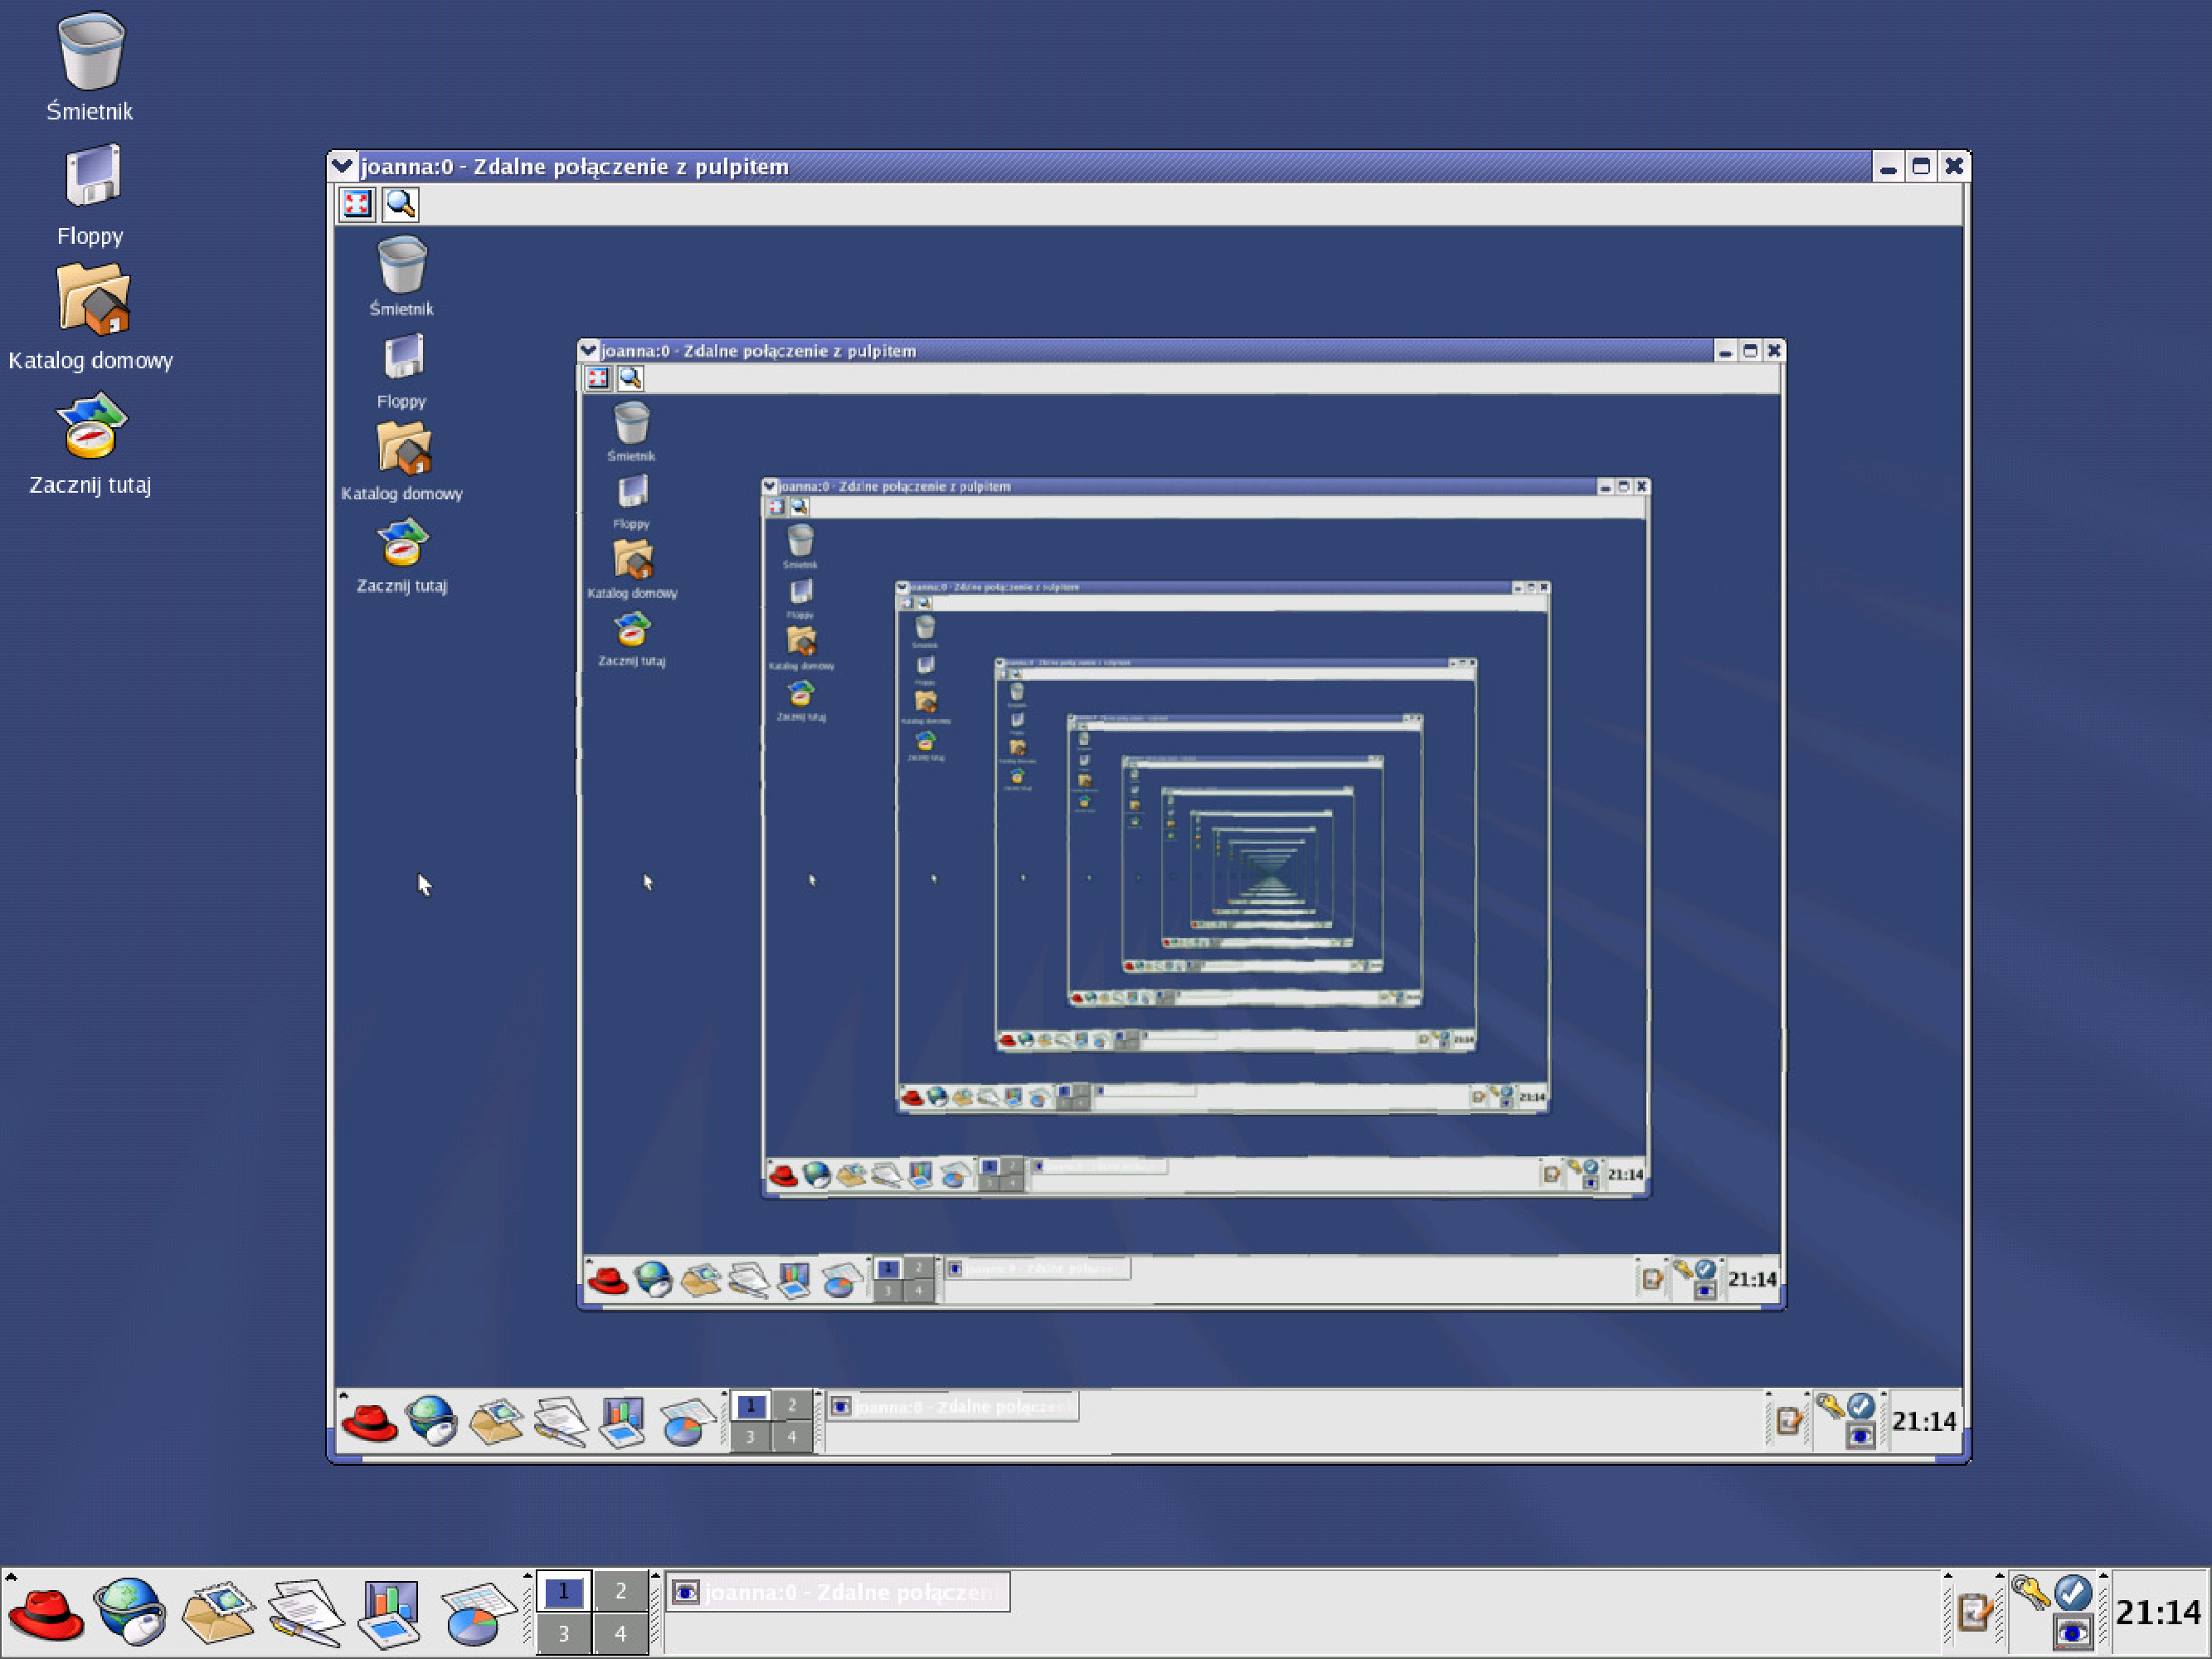
\includegraphics[width=10cm]{graficos/recursive}
\figcaption{Otra imagen recursiva: captura de pantalla de RedHat.}%
\label{fig:redhat_recursivo}%
\end{minipage}

\section{Algoritmos recursivos y algoritmos iterativos}

Llamaremos {\it algoritmos recursivos} a aquellos que realizan llamadas
recursivas para llegar al resultado, y {\it algoritmos iterativos} a
aquellos que llegan a un resultado a través de una iteración mediante un
ciclo definido o indefinido.

Todo algoritmo recursivo puede expresarse como iterativo y viceversa.  Sin
embargo, según las condiciones del problema a resolver podrá ser preferible
utilizar la solución recursiva o la iterativa.

Una posible implementación iterativa de la función \lstinline!factorial!
vista anteriormente sería:

\begin{codigo-python-sn}
def factorial(n):
    """Precondición: n entero >= 0
       Devuelve: n!"""
    fact = 1
    for num in range(n, 1, -1):
        fact *= num
    return fact
\end{codigo-python-sn}

Se puede ver que en este caso no es necesario incluir un caso base, ya que
el mismo ciclo incluye una condición de corte, pero que sí es necesario
incluir un acumulador, que en el caso recursivo no era necesario.

Por otro lado, si hiciéramos el seguimiento de esta función, como se hizo
para la versión recursiva, veríamos que la pila de ejecución siempre tiene un
único marco, en el cual se van modificando los valores de \lstinline!num! y
\lstinline!fact!.

Es por esto que, en general, las versiones recursivas de los algoritmos
utilizan más memoria (ya que la pila de ejecución se guarda en
memoria) pero suelen ser más elegantes.

\section{Un ejemplo de recursión elegante}

Consideremos ahora otro problema que puede ser resuelto de forma elegante
mediante un algoritmo recursivo.

La función \lstinline!potencia(b, n)!, vista en unidades anteriores,
realizaba \lstinline!n! iteraciones para poder obtener el valor de $b^n$.
Sin embargo, es posible optimizarla teniendo en cuenta que:

\begin{align*}
b^n &= b^{n/2} \cdot b^{n/2} &&\text{si}\;n\;\text{es par.} \\
b^n &= b^{(n-1)/2} \cdot b^{(n-1)/2} \cdot b &&\text{si}\;n\;\text{es impar.} \\
\end{align*}

Antes de programar cualquier función recursiva es necesario decidir cuál
será el {\it caso base} y cuál el {\it caso recursivo}.  Para esta función,
tomaremos $n=0$ como el caso base, en el que devolveremos $1$; y el caso
recursivo tendrá dos partes, correspondientes a los dos posibles grupos de
valores de $n$.

\begin{codigo-python-sn}
def potencia(b,n):
    """Precondición: n >= 0
       Devuelve: b^n."""

    if n <= 0:
        # caso base
        return 1

    if n % 2 == 0:
        # caso n par
        p = potencia(b, n / 2)
        return p * p
    else:
        # caso n impar
        p = potencia(b, (n-1)/2)
        return p * p * b
\end{codigo-python-sn}

El uso de la variable \lstinline!p! en este caso no es optativo, ya que
es una de las ventajas principales de esta implementación: se aprovecha el
resultado calculado en lugar de tener que calcularlo dos veces. Vemos que
este código funciona correctamente:

\begin{codigo-python-sn}
>>> potencia(2, 10)
1024
>>> potencia(3, 3)
27
>>> potencia(5, 0)
1
\end{codigo-python-sn}

El orden de las llamadas, haciendo un seguimiento simplificado de la
función será:

\begin{enumerate}
\item \verb!potencia(2, 10)!
\item \hspace{1cm} \verb!p = potencia(2, 5) !
\hspace{4cm} \begin{tabular}{|c|c|}\verb|b| $\rightarrow$ 2 & \verb|n| $\rightarrow$ 10\end{tabular}
\item \hspace{2cm} \verb!p = potencia(2, 2) !
\hspace{3cm} \begin{tabular}{|c|c|}\verb|b| $\rightarrow$ 2 & \verb|n| $\rightarrow$ 5$\;\,$\end{tabular}
\item \hspace{3cm} \verb!p = potencia(2, 1) !
\hspace{2cm} \begin{tabular}{|c|c|}\verb|b| $\rightarrow$ 2 & \verb|n| $\rightarrow$ 2$\;\,$\end{tabular}
\item \hspace{4cm} \verb!p = potencia(2, 0) !
\hspace{1cm} \begin{tabular}{|c|c|}\verb|b| $\rightarrow$ 2 & \verb|n| $\rightarrow$ 1$\;\,$\end{tabular}
\item \hspace{5cm} \verb!return 1           !
\hspace{0cm} \begin{tabular}{|c|c|}\verb|b| $\rightarrow$ 2 & \verb|n| $\rightarrow$ 0$\;\,$\end{tabular}
\item \hspace{4cm} \verb!return 1 * 1 * 2   !
\hspace{1cm} \begin{tabular}{|c|c|c|}\verb|b| $\rightarrow$ 2 & \verb|n| $\rightarrow$ 1$\;\,$
& \verb|p| $\rightarrow$ 1$\;\,$ \end{tabular}
\item \hspace{3cm} \verb!return 2 * 2       !
\hspace{2cm} \begin{tabular}{|c|c|c|}\verb|b| $\rightarrow$ 2 & \verb|n| $\rightarrow$ 2$\;\,$
& \verb|p| $\rightarrow$ 2$\;\,$ \end{tabular}
\item \hspace{2cm} \verb!return 4 * 4 * 2   !
\hspace{3cm} \begin{tabular}{|c|c|c|}\verb|b| $\rightarrow$ 2 & \verb|n| $\rightarrow$ 5$\;\,$
& \verb|p| $\rightarrow$ 4$\;\,$ \end{tabular}
\item \hspace{1cm} \verb!return 32 * 32     !
\hspace{4cm} \begin{tabular}{|c|c|c|}\verb|b| $\rightarrow$ 2 & \verb|n| $\rightarrow$ 10
& \verb|p| $\rightarrow$ 32 \end{tabular}
\end{enumerate}

Se puede ver, entonces, que para calcular $2^{10}$ se realizaron 5 llamadas a
\lstinline!potencia!, mientras que en la implementación más sencilla se
realizaban 10 iteraciones. Y esta optimización será cada vez más importante
a medida que aumenta \lstinline!n!: por ejemplo para $n = 100$ se
realizarán 8 llamadas recursivas, y para $n = 1000$ 11 llamadas.

% Esto no es para darlo, es sólo para que esté

Para transformar este algoritmo recursivo en un algoritmo iterativo, es
necesario {\it simular} la pila de llamadas a funciones mediante una pila que
almacene los valores que sean necesarios.  En este caso, lo que apilaremos será
si el valor de \lstinline!n! es par o no.

\begin{codigo-python-sn}
def potencia(b, n):
    """Precondición: n >= 0
       Devuelve: b^n."""

    pila = []
    while n > 0:
        if n % 2 == 0:
            pila.append(True)
            n /= 2
        else:
            pila.append(False)
            n = (n - 1) / 2

    p = 1
    while pila:
        es_par = pila.pop()
        if es_par:
            p *= p
        else:
            p *= p * b

    return p
\end{codigo-python-sn}

Como se puede ver, este código es mucho más complejo que la versión recursiva.
Esto se debe a que utilizando recursión el uso de la pila de llamadas a
funciones oculta el proceso de apilado y desapilado y permite concentrarse
en la parte importante del algoritmo.

\section{Un ejemplo de recursión poco eficiente}

Del ejemplo anterior se podría deducir que siempre es mejor utilizar algoritmos
recursivos; sin embargo ---como ya se dijo--- cada situación debe ser analizada por
separado.

Un ejemplo clásico en el cual la recursión tiene un resultado muy poco
eficiente es el de los números de Fibonacci.  La sucesión de Fibonacci está
definida por la siguiente relación:

\begin{align*}
F_n &= 0 &&\text{si}\;n = 0\\
F_n &= 1 &&\text{si}\;n = 1\\
F_n &= F_{n - 1} + F_{n - 2} &&\text{si}\;n > 1
\end{align*}

Los primeros números de esta sucesión son: $0$, $1$, $1$, $2$, $3$, $5$, $8$,
$13$, $21$, $34$, $55$.

Dada la definición recursiva de la sucesión, puede resultar muy tentador
escribir una función que calcule en valor de \lstinline!fib(n)! de la siguiente
forma:

\begin{codigo-python-sn}
def fib(n):
    """Precondición: n >= 0.
       Devuelve: el número de Fibonacci número n."""
    if n == 0 or n == 1:
        return n
    return fib(n - 1) + fib(n - 2)
\end{codigo-python-sn}

Si bien esta implementación es muy sencilla y elegante, también es extremadamente
poco eficiente: para calcular \lstinline!fib(n - 1)! es necesario calcular
\lstinline!fib(n - 2)!, que luego volverá a ser calculado para obtener el valor
\lstinline!fib(n)!.

Por ejemplo, una simple llamada a \lstinline!fib(5)!, generaría
recursivamente todas las llamadas ilustradas en la Figura \ref{fibonacci}.
Puede verse que muchas de estas llamadas están repetidas, generando un
total de 15 llamadas a la función \lstinline!fib!, sólo para devolver el
valor $F_5$.

\begin{figure}[htb]
\includegraphics{graficos/18_fibonacci}
\caption{Árbol de llamadas para \lstinline!fib(5)!}
\label{fibonacci}
\end{figure}

En este caso, será mucho más conveniente utilizar una versión iterativa,
que vaya almacenando los valores de las dos variables anteriores a medida
que los va calculando.

\begin{codigo-python-sn}
def fib(n):
    """Precondición: n >= 0.
       Devuelve: el número de Fibonacci número n."""
    if n == 0 or n == 1:
        return n
    ant2 = 0
    ant1 = 1
    for i in range(2, n + 1):
        fibn = ant1 + ant2
        ant2 = ant1
        ant1 = fibn
    return fibn
\end{codigo-python-sn}

Vemos que el caso base es el mismo para ambos algoritmos, pero que en el
caso iterativo se calcula el número de Fibonacci de forma incremental, de
modo que para obtener el valor de \lstinline!fib(n)! se harán $n-1$
iteraciones.

\begin{atencion}
En definitiva, vemos que un algoritmo recursivo {\bf no} es mejor que uno
iterativo, ni viceversa.  En cada situación será conveniente analizar cuál
algoritmo provee la solución al problema de forma más clara y eficiente.
\end{atencion}

\section{Limitaciones}

Si creamos una función sin {\it caso base}, obtendremos el equivalente
recursivo de un bucle infinito.  Sin embargo, como cada llamada recursiva
agrega un elemento a la pila de llamadas a funciones y la memoria de
nuestras computadoras no es infinita, el ciclo deberá terminarse cuando se
agote la memoria disponible.

En particular, en Python, para evitar que la memoria se termine, la pila de
ejecución de funciones tiene un límite. Es decir, que si se ejecuta un
código como el que sigue:

\begin{codigo-python-sn}
def inutil(n):
    return inutil(n - 1)
\end{codigo-python-sn}

Se obtendrá un resultado como el siguiente:

\begin{codigo-python-sn}
>>> inutil(1)
  File "<stdin>", line 2, in inutil
  File "<stdin>", line 2, in inutil
  (...)
  File "<stdin>", line 2, in inutil
RecursionError: maximum recursion depth exceeded
\end{codigo-python-sn}

El límite por omisión es de 1000 llamadas recursivas. Es posible modificar
el tamaño máximo de la pila de recursión mediante la instrucción
\lstinline!sys.setrecursionlimit(n)!.  Sin embargo, si se está alcanzando
este límite suele ser una buena idea pensar si realmente el algoritmo
recursivo es el que mejor resuelve el problema.

\begin{sabias_que}
Existen algunos lenguajes {\it funcionales}, como Haskell, ML, o Scheme, en
los cuales la recursión es la única forma de realizar un ciclo.  Es
decir, no existen construcciones |while| ni |for|.

Estos lenguajes cuentan con una optimización especial, llamada {\it
optimización de recursión por cola} ({\it tail recursion optimization}),
que permite que cuando una función realiza su llamada recursiva como {\it
última} acción antes de terminar, no se apile el estado de la función
innecesariamente, evitando el consumo adicional de memoria mencionado
anteriormente.

La función \lstinline!factorial! vista en esta unidad es un ejemplo de {\it
recursión por cola} cuya ejecución podría ser optimizada por el compilador o
intérprete del lenguaje.
\end{sabias_que}

\section{Resumen}

\begin{itemize}

\item A medida que se realizan llamadas a funciones, el estado cada
función se almacena en la {\it pila de ejecución}.

\item Esto permite que sea posible que una función se llame a sí misma,
pero que las variables dentro de la función tomen distintos valores.

\item La {\bf recursión} es el proceso en el cual una función se invoca a
sí misma.  Este proceso permite crear un nuevo tipo de ciclos.

\item Siempre que se escribe una función recursiva es importante considerar
el {\bf caso base} (el que detendrá la recursión) y el {\bf caso
recursivo} (el que realizará la llamada recursiva).  Una función recursiva
sin caso base es equivalente a un bucle infinito.

\item Una función no es mejor ni peor por ser recursiva.  En cada situación
a resolver puede ser conveniente utilizar una solución recursiva o una
iterativa.  Para elegir una o la otra será necesario analizar las
características de elegancia y eficiencia.

\end{itemize}


\newpage
\section{Ejercicios}

\extractionlabel{guia}
\begin{ejercicio}
Escribir una función que reciba un número positivo $n$ y devuelva
la cantidad de dígitos que tiene.
\end{ejercicio}

\extractionlabel{guia}
\begin{ejercicio}
Escribir una función que simule el siguiente experimento:
Se tiene una rata en una jaula con 3 caminos, entre los cuales elige
al azar (cada uno tiene la misma probabilidad), si elige el {\it 1} luego
de 3 minutos vuelve a la jaula, si elige el {\it 2} luego de 5 minutos vuelve a
la jaula, en el caso de elegir el {\it 3} luego de 7 minutos sale de la jaula.
La rata no aprende, siempre elige entre los 3 caminos con la misma probabilidad,
pero quiere su libertad, por lo que recorrerá los caminos hasta salir de la jaula.

La función debe devolver el tiempo que tarda la rata en salir de la jaula.
\end{ejercicio}

\extractionlabel{guia}
\begin{ejercicio}
Escribir una función que reciba 2 enteros {\it n} y {\it b} y devuelva
\verb!True! si {\it n} es potencia de {\it b}.

Ejemplos:
\begin{verbatim}
>>> es_potencia(8,2)
True
>>> es_potencia(64,4)
True
>>> es_potencia(70,10)
False
\end{verbatim}
\end{ejercicio}

\extractionlabel{guia}
\begin{ejercicio}
Escribir una funcion recursiva que reciba como parámetros dos strings {\it a} y
{\it b}, y devuelva una lista con las posiciones en donde se encuentra {\it b}
dentro de {\it a}.

Ejemplo:
\begin{verbatim}
>>> posiciones_de("Un tete a tete con Tete", "te")
[3, 5, 10, 12, 21]
\end{verbatim}
\end{ejercicio}

\extractionlabel{guia}
\begin{ejercicio}
Escribir dos funciones mutualmente recursivas par(n) e impar(n) que
determinen la paridad del numero natural dado, conociendo solo que:
\begin{itemize}
    \item 1 es impar.
    \item Si un número es impar, su antecesor es par; y viceversa.
\end{itemize}
\end{ejercicio}

\extractionlabel{guia}
\begin{ejercicio}
Escribir una función que calcule recursivamente el n-ésimo número
triangular (el número 1 + 2 + 3 + ... + n).
\end{ejercicio}

\extractionlabel{guia}
\begin{ejercicio}
Escribir una función que calcule recursivamente cuántos elementos
hay en una pila, suponiendo que la pila sólo tiene los métodos apilar
y desapilar, y no altere el contenido de la pila.\\
¿Implementarías esta función para un programa real? ¿Por qué?
\end{ejercicio}

\extractionlabel{guia}
\begin{ejercicio}
Escribir una funcion recursiva que encuentre el mayor elemento de una lista.
\end{ejercicio}

\extractionlabel{guia}
\begin{ejercicio}
Escribir una función recursiva para replicar los elementos de una lista
una cantidad n de veces. Por ejemplo,
\verb!replicar ([1, 3, 3, 7], 2) = ([1, 1, 3, 3, 3, 3, 7, 7])!
\end{ejercicio}

